\documentclass[handout]{beamer}

\usetheme[progressbar=frametitle]{metropolis}
\metroset{block=fill}

\subtitle{NTIN071 Automata and Grammars}
\author{Jakub Bulín (KTIML MFF UK)}

\date{Spring 2025\\ 
    \vspace{1in} 
    \begin{flushleft}
        \it \footnotesize * Adapted from the Czech-lecture slides by Marta Vomlelová with gratitude. The translation, some modifications, and all errors are mine.
    \end{flushleft}
}

%% packages

\usepackage{amsmath}
\usepackage{amssymb}
\usepackage{amsthm}
\usepackage{cancel}
\usepackage{color}
\usepackage{colortbl}
\usepackage{forest}
\usepackage[utf8x]{inputenc}
\usepackage{multicol}
\usepackage{multirow}

%% colors
\definecolor{Gray}{gray}{0.9}

%% TikZ
\usepackage{tikz}
    \usetikzlibrary{
        automata,
        arrows,
        backgrounds,
        decorations.pathmorphing,
        fit,
        positioning,
        shapes,
        shapes.geometric,
        tikzmark
    } 
    \tikzset{>=stealth',shorten >=1pt,auto,node distance=2cm}
    \tikzset{initial text={}}
    \tikzset{elliptic state/.style={draw,ellipse}}

%% amsthm
\theoremstyle{plain}
    \newtheorem*{algorithm}{Algorithm}    
    \newtheorem*{observation}{Observation}
    \newtheorem*{proposition}{Proposition}

\theoremstyle{remark}
    \newtheorem*{exercise}{Exercise}
    \newtheorem*{remark}{Remark}

%% macros
\DeclareMathOperator{\RegE}{RegE}
\DeclareMathOperator{\RL}{RL}

% Just for Lecture 2
\newcommand{\x}{$\times$}
\newcommand{\nx}{\ }



\title{Lecture 8 -- Equivalence of PDA and CFG, Deterministic PDA}


\begin{document}


\frame{\titlepage}


\begin{frame}{Recap of Lecture 7}
	
    \begin{itemize}    
        \item Testing membership in a context-free language: the Cocke-Younger-Kasami algorithm
        \item Testing emptiness and finiteness of a context-free language    
		\item Pushdown automaton: extend an $\epsilon$-NFA with a stack memory (potentially infinite), pop the top symbol, decide based on $(q,a,X)$, can push a finite string of stack symbols
        \item Acceptance by final state $L(P)$ and by empty stack $N(P)$, conversion between the two options        	
	\end{itemize}

\end{frame}



\section*{2.10 Equivalence of PDA and context-free grammars}


\begin{frame}{Equivalence of PDA and CFG}

    \begin{theorem}
        The following statements about $L\subset\Sigma^*$ are equivalent:
        \begin{enumerate}[(i)]
            \item There exists a context-free grammar such that $L(G)=L$.
            \item There exists a PDA such that $L(P)=L$.
            \item There exists a PDA such that $N(P)=L$.
        \end{enumerate}
    \end{theorem}
        
    \begin{center}
        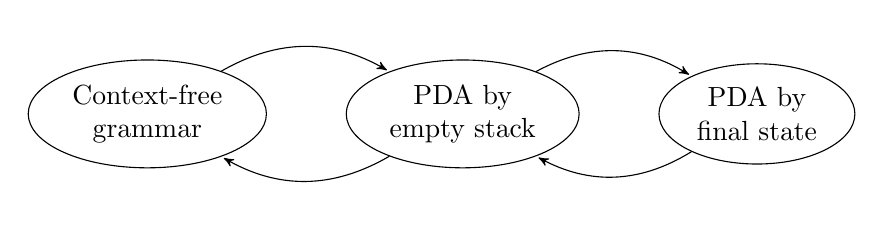
\begin{tikzpicture}
            \node[elliptic state][align=center] (p)      {Context-free\\ grammar};
            \node[elliptic state][align=center] (q) [right=1cm of p]     {PDA by\\empty stack};
            \node[elliptic state][align=center] (r) [right=1cm  of q]     {PDA by\\final state};
            \path[->]
                (p)  edge[bend left] node {} (q)
                (q)  edge[bend left] node {} (p)
                (q)  edge[bend left] node {} (r)
                (r)  edge[bend left] node {} (q)
            ;
        \end{tikzpicture}    
    \end{center}

    We have already shown $(ii)\Leftrightarrow(iii)$. To prove equivalence with a context-free grammar, we use acceptance by empty stack.

\end{frame}


\section*{Context-free grammar to pushdown automaton}


\begin{frame}{CFG to PDA}

    \begin{block}{The construction}
        Given $G=(V,T,\mathcal P,S)$, construct $P=(\{q\},T,V\cup T,\delta,q,S)$:
        \begin{enumerate}[(1)]
            \item for each $ A\in V$, \alert{$\delta(q,\epsilon, A)=\{(q,\beta)\mid A\rightarrow \beta \in\mathcal P\}$} \\ \hfill [apply rule]
            \item for each $a\in T$, \alert{$\delta(q,a,a)=\{(q,\epsilon)\}$}\\ \hfill [match terminal]
        \end{enumerate}   
    \end{block} 

    \textbf{How it works:}
    \begin{itemize}
        \item a \alert{leftmost} derivation is simulated by the PDA
        \item current sentential form = part of input read + stack contents
        \item see a variable: apply rule, a terminal: read \& pop from stack
    \end{itemize}

\end{frame}


\begin{frame}{An example}

    \begin{example}
        $I\rightarrow a\mid b\mid Ia\mid Ib\mid I0\mid I1$,\\
        $E\rightarrow I\mid E*E\mid E+E\mid (E)$
    \end{example}
        
    $\Sigma=\{a,b,0,1,(,),+,*\}$, $\Gamma=\Sigma\cup\{I,E\}$,  $\delta$ is defined as follows:

    \begin{itemize}
        \item $\delta(q,\epsilon,I)=\{(q,a),(q,b),(q,Ia),(q,Ib),(q,I0),(q,I1)\}$
        \item $\delta(q,\epsilon,E)=\{(q,I),(q,E*E),(q,E+E),(q,(E))\}$
        \item $\delta(q,s,s)=\{(q,\epsilon)\}$ for all $s\in \Sigma$ (e.g. $\delta(q,+,+)=\{(q,\epsilon)\}$)
        \item $\delta(q,x)$ is empty otherwise
    \end{itemize}

    \alert{Leftmost derivation:} $E\Rightarrow E*E\Rightarrow I*E\Rightarrow a*E\Rightarrow a*I\Rightarrow a*b$\\       	
    
    \medskip

    The sequence of configurations:

    $(q,a*b,E)$
    $\vdash$ $(q,a*b,E*E)$
    $\vdash$ $(q,a*b,I*E)$
    $\vdash$ $(q,a*b,a*E)$
    $\vdash$ $(q,*b,*E)$
    $\vdash$ $(q,b,E)$
    $\vdash$ $(q,b,I)$
    $\vdash$ $(q,b,b)$
    $\vdash$ $(q,\epsilon,\epsilon)$

\end{frame}


\begin{frame}{Proof that $N(P)=L(G)$\hfill \alert{(i) $w\in L(G)\Rightarrow w\in N(P)$}}

    Start with a leftmost derivation $S=\gamma_1\Rightarrow_{lm}\ldots\Rightarrow_{lm}\gamma_n=w$.

    Prove by induction on $i$ that $(q,w,S)\vdash_P^* (q, v_i,\alpha_i)$, where $\gamma_i=u_i\alpha_i$ is the $i$-th sentential form and $u_iv_i=w$.

    If $\gamma_i$ contains only terminals, set $\gamma_i=w=u_i, v_i=\epsilon=\alpha_i$. Otherwise, write $\gamma_i=u_iA\alpha_i$, where $u_i\in T^*$ and $A\in V$ is the leftmost variable.

    By induction we have $(q,w,S)\vdash_P^* (q, v_i,A\alpha_i)$, $w=u_iv_i$.

    For the step $\gamma_i\Rightarrow_{lm}\gamma_{i+1}$ we used some rule $A\rightarrow\beta\in P$. The PDA replaces $A$ on the stack with $\beta$, moves to configuration $(q,v_i,\beta\alpha_i)$.

    We pop all terminals $v\in \Sigma^*$ from the beginning of $\beta\alpha$ (matching them with the input): $v_i=vv_{i+1}$ and $\beta\alpha=v\alpha_{i+1}$

    We got to $(q,v_{i+1},\alpha_{i+1})$, corresponds to the sentential form $\gamma_{i+1}$.
    
\end{frame}


\begin{frame}{Proof that $N(P)=L(G)$\hfill \alert{(ii) $w\in N(P)\Rightarrow w\in L(G)$}}

    \vspace{-3pt}
    Prove that if $(q,u,X)\vdash_P^*(q,\epsilon,\epsilon)$, then $X\Rightarrow_G^* u$. By induction on the number of moves. \textbf{Basis} \alert{$n=1$} move:
    \begin{itemize}
        \item $X=a\in\Sigma$: $\delta(q, a, a)\ni (q,\epsilon)$, $u=a$, 0-step derivation
        \item $X=A\in \Gamma$: $\delta(q,\epsilon,A)\ni (q,\epsilon)$ coming from $A\rightarrow\epsilon\in\mathcal P$, $u=\epsilon$
    \end{itemize} 

    \vspace{-3pt}
    \textbf{Induction step} \alert{$n>1$} moves: if the first move is \alert{[match terminal]}, don't extend the derivation, if it is \alert{[apply rule]}: $A$ on top of stack was replaced by $\beta=Y_1Y_2\ldots Y_k$, for a rule $A\to\beta\in\mathcal P$.

    \begin{columns}

        \column{0.78\textwidth}
    
        Split $u=u_1\ldots u_k$ s.t. while popping $Y_i$ we read~$u_i$, i.e. $(q,u_iu_{i+1}\ldots u_k,Y_i)\vdash^*(q,u_{i+1}\ldots u_k,\epsilon)$

        \medskip
        
        Thus also $(q,u_i,Y_i)\vdash^*(q,\epsilon,\epsilon)$, by induction assumption we get $Y_i\Rightarrow^*u_i$. Together:
        {\small
        $$
        A\Rightarrow Y_1Y_2\ldots Y_k\Rightarrow^* u_1Y_2\ldots Y_k\Rightarrow^* \ldots \Rightarrow^* u_1u_2\ldots u_k
        $$
        } 
        
        \vspace{-6pt}\hfill\qedsymbol
    
        \column{0.22\textwidth}

        \scalebox{0.85}{
            \input{files/PDACFG.pdf_t}
        }
        
    \end{columns}    
       
\end{frame}


\section*{Pushdown automaton to context-free grammar}


\begin{frame}{An example}

    \begin{columns}

        \column{0.7\textwidth}\centering
        
        Given $P=(\{q\},\{\mathtt{if},\mathtt{else}\},\{Z\},\delta,q,Z)$
        
        \smallskip

        $\delta(q,\mathtt{if},Z)=\{(q,ZZ)\}$\\        
        $\delta(q,\mathtt{else},Z)=\{(q,\epsilon)\}$
        
        \column{0.3\textwidth}

        \begin{center}
            \scalebox{0.9}{
                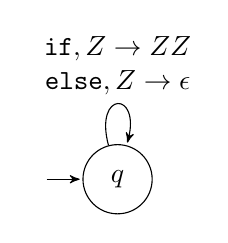
\begin{tikzpicture}
                    \node[initial,state] (q) {$q$};
                    \path[->]
                        (q)  edge[loop above] node[align=center] { $\mathtt{if},Z\rightarrow ZZ$\\ $\mathtt{else},Z\rightarrow \epsilon$} (q);
                \end{tikzpicture}
            }
        \end{center} 

    \end{columns}

    Construct $G=(V,\{\mathtt{if},\mathtt{else}\},\mathcal P,S)$

    \begin{itemize}
        \item variables: $V=\{S,[qZq]\}$ 
        \item production rules:
        \begin{itemize}
            \item $S\rightarrow [qZq]$            
            \item $[qZq]\rightarrow \mathtt{else}$
            \item $[qZq]\rightarrow \mathtt{if}[qZq][qZq]$
            
        \end{itemize}        
    \end{itemize}    
    
    In this example, $S$ and $[qZq]$ generate the same words, so we can simplify:
         $G=(\{S\},\{\mathtt{if},\mathtt{else}\},\{S\rightarrow \mathtt{if}SS\mid\mathtt{else}\},S)$
    
\end{frame}


\begin{frame}{PDA to CFG: the construction}

    \vspace{-6pt}
    \begin{itemize}
        \item key event: pop a symbol $X$, while changing from state $q$ to $r$
        \item variables: $[qXr]$ for $q,r\in Q$ and $X\in \Gamma$, plus a new variable~$S$
        $$
        L([qXr])=\{w\in\Sigma^*\mid (q,w,X)\vdash_P^*(r,\epsilon,\epsilon)\}
        $$
        \item $S$ to choose (guess) in which state the stack is emptied
    \end{itemize}

    \begin{block}{The construction}
        Given $P=(Q,\Sigma,\Gamma,\delta,q_0,Z_0)$, construct $G=(V,T,\mathcal P,S)$ where $V=\{S\}\cup\{[pXq]\mid p,q\in Q,X\in\Gamma\}$ and the productions are:   
        \begin{enumerate}[(i)]
            \item for every state $p\in Q$ add $S\to [q_0Xp]$ 
            \item for every transition $({\color{red}p},Y_1Y_2\ldots Y_k)\in\delta({\color{red}q,a,X})$ (incl. $a=\epsilon$) and \alert{all $k$-tuples of states} $p_1,\dots,p_{k-1},{\color{blue}p_k}\in Q$ add
            
            \vspace{-6pt}
            $$
            [{\color{red}qX}{\color{blue}p_k}]\rightarrow {\color{red}a}[{\color{red}p}Y_1p_1][p_1Y_2p_2]\ldots [p_{k-1}Y_k{\color{blue}p_k}]
            $$                  
        \end{enumerate}        
        %\vspace{-3pt}      
        In particular, for $(p,\epsilon)\in\delta(q,a,X)$ (i.e., $k=0$) add $[qXp]\rightarrow a$.
    \end{block}

\end{frame}


\begin{frame}{Another example: $\{0^n1^n\mid n>0\}$}

    \vspace{-6pt}
    {\small    
        \begin{center}
            \begin{tabular}{l l c}
                $\delta$ & Productions & \\\hline
                & $S\rightarrow [pZp]\mid [pZq]$ & (1)\\
                $\delta(p,0,Z)\ni (p,A)$	& $[pZp]\rightarrow 0[pAp] $ & (2)\\
                & $[pZq]\rightarrow 0[pAq] $& (3)\\
                $\delta(p,0,A)\ni (p,AA)$ & $[pAp]\rightarrow 0[pAp][pAp]$ & (4)\\
                & $[pAp]\rightarrow 0[pAq][qAp] $ & (5)\\
                & $[pAq]\rightarrow 0[pAp][pAq] $ & (6)\\
                & $[pAq]\rightarrow 0[pAq][qAq] $ & (7)\\
                $\delta(p,1,A)\ni (q,\epsilon)$ & $[pAq]\rightarrow 1$ & (8)\\			
                $\delta(q,1,A)\ni (q, \epsilon)$ & $[qAq]\rightarrow 1$ & (9)			
            \end{tabular}
        \end{center}
    }

    \bigskip

    \begin{columns}

        \column{0.5\textwidth}

        Derivation of $0011$:\vspace{-12pt}
        \begin{align*}
            S &\Rightarrow^{(1)} [pZq] \Rightarrow^{(3)} 0[pAq]\\
              &\Rightarrow^{(7)} 00[pAq][qAq]\\
              &\Rightarrow^{(8)} 001[qAq]\Rightarrow^{(9)} 0011   
        \end{align*}

        \column{0.5\textwidth}

        \begin{center}
            \scalebox{0.9}{
                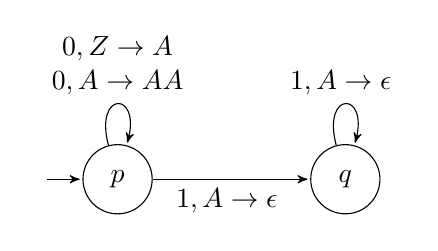
\begin{tikzpicture}
                    \node[initial,state] (p)      {$p$};
                    \node[state] (q)  [right=2cm of p]     {$q$};
                    \path[->]
                        (p)  edge[loop above]  node[align=center] {
                            $0,Z \rightarrow A$	\\
                            $0,A \rightarrow AA$	
                        } (p)
                        (p)  edge[swap]  node[align=center] {
                            $1,A \rightarrow \epsilon$			
                        }  (q)
                        (q)  edge[loop above]  node[align=center] {
                            $1,A \rightarrow \epsilon$			
                        } (q);           
                \end{tikzpicture}                
            }
        \end{center}

    \end{columns}

\end{frame}


\begin{frame}{Sketch of proof that $L(G)=N(P)$}

    \begin{columns}

        \column{0.7\textwidth}

        It suffices to show that:
        $$
        [qXp]\Rightarrow^*w\ \text{ iff }\ (q,w,X)\vdash^*(p,\epsilon,\epsilon)
        $$

        In both directions, the proof is done by induction (number of moves/steps).
        
        \column{0.3\textwidth}

        \begin{center}
            \input{files/PDACFG2.pdf_t}    
        \end{center}

        \hfill\qedsymbol
                
    \end{columns}

\end{frame}


\section*{2.11 Deterministic pushdown automata}


\begin{frame}{The definition}

    \begin{definition}[Deterministic PDA]
        A pushdown automaton $P=(Q,\Sigma,\Gamma,\delta,q_0,Z_0,F)$ is \alert{deterministic} (a \alert{DPDA}) iff both of the following hold:
        \begin{enumerate}[(i)]
            \item The set of possible transitions $\delta(q,a,X)$ is at most one-element for all  $q\in Q$, $a\in\Sigma \cup \{\epsilon\}$, and $X\in\Gamma$.
            \item If $\delta(q,a,X)\neq\emptyset$ for some $a\in \Sigma$, then $\delta(q,\epsilon,X)=\emptyset$.
        \end{enumerate}    
    \end{definition}

    A language $L$ is a \alert{deterministic} context-free language, if $L=L(P)$ for some DPDA $P$.

\end{frame}


\begin{frame}{Example: even palindromes with a center mark}

    \vspace{-3pt}
    $L_{wwr}=\{ww^R\mid w\in\{0,1\}^*\}$ is context free, but not recognizable by a DPDA [proof coming soon]; (ii) forbids a choice between an $\epsilon$-transition and reading the next input symbol.
    
    But if we put in a `center mark' $c$, $L_{wcwr}=\{wcw^R\mid w\in\{0,1\}^*\}$ is recognized by the following DPDA:
        
    \begin{center}
        \scalebox{0.83}{
            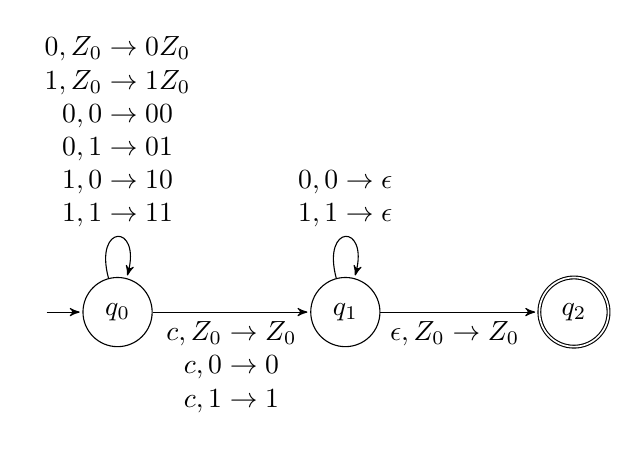
\begin{tikzpicture}
                \node[initial,state] (q0)      {$q_0$};
                \node[state] (q1)  [right=2cm of q0]     {$q_1$};
                \node[state, accepting] (q2)  [right=2cm of q1]    {$q_2$};
                \path[->]
                    (q0)  edge[loop above]  node[align=center] {
                        $0,Z_0 \rightarrow 0Z_0$	\\
                        $1,Z_0 \rightarrow 1Z_0$	\\			
                        $0,0 \rightarrow 00$	\\			
                        $0,1 \rightarrow 01$	\\			
                        $1,0 \rightarrow 10$	\\			
                        $1,1 \rightarrow 11$			
                        } (q0)
                    (q0)  edge[swap]  node[align=center] {
                        $c,Z_0 \rightarrow Z_0$	\\			
                        $c,0 \rightarrow 0$	\\			
                        $c,1 \rightarrow 1$			
                        }  (q1)
                    (q1)  edge[loop above]  node[align=center] {
                        $0,0 \rightarrow \epsilon$	\\			
                        $1,1 \rightarrow \epsilon$			
                        } (q1)
                    (q1)  edge[swap]  node[align=center] {
                        $\epsilon,Z_0 \rightarrow Z_0$	
                        } (q2)
                    ;    
            \end{tikzpicture}
        }
    \end{center}

\end{frame}


\begin{frame}{Languages recognized by deterministic PDA}

    \vspace{-24pt}
    {\Large
    $$
    RL\subsetneq L_{DPDA} \subsetneq L_{PDA}=CFL = N_{PDA}\supsetneq N_{DPDA}
    $$
    }
    \vspace{-6pt}
      
    \begin{proposition}
        For every regular language $L$, there is a DPDA $P$ with $L=L(P)$.
    \end{proposition}

    \vspace{-6pt}
    DPDA can simulate a DFA, ignore the stack (leave $Z_0$ on top).
    \hfill\qedsymbol
 
    \medskip

    \begin{example}
       $L_{wcwr}$ is recognized by a DPDA by final state, but not regular.
    \end{example}

    \vspace{-6pt}
    DPDA on the previous slide, nonregularity by PL for $z=0^nc0^n$.
    \hfill\qedsymbol

    \medskip
    
    \begin{example}
        $L=\{a^ib^i\mid i \in \mathbb{N}\} \cup \{a^ib^{2i}\mid i \in \mathbb{N}\}$ is context-free, but not recognizable by any DPDA by final state.
    \end{example}

    \vspace{-6pt}
    Context-freeness is easy. Not in $L_{DPDA}$: next slide.

\end{frame}


\begin{frame}{$L_{abb}=\{a^ib^i|i \in \mathbb{N}\} \cup \{a^ib^{2i}|i \in \mathbb{N}\}\notin L_{DPDA}$}

    \vspace{-3pt}
    Assume for contradiction: recognized by a DPDA $M$ by final state.
    Create two copies, $M_1$ and $M_2$, call corresponding nodes `siblings'. Construct a (nondeterministic) PDA $M'$:
    
    \vspace{-3pt}
    \begin{itemize}
        \item initial state: the initial state of $M_1$
        \item final states: the final states of $M_2$
        \item \alert{reroute transitions} going out of final states of $M_1$ to the siblings in $M_2$, relabel $b$ to $c$ (e.g. $\delta(f,b,X)=\{(q,X)\}$ becomes $\delta(f,c,X)=\{(q',X)\}$ where $q'$ is the sibling of $q$)
        \item in the automaton $M_2$, \alert{relabel} $b$-transitions to $c$-transitions 
    \end{itemize}

    \vspace{-3pt}
    The resulting PDA $M'$ recognizes \alert{$\{a^ib^ic^i\mid i \in \mathbb{N}\}$} by final state: determinism of $M$ means a \alert{unique path} when reading $a^ib^{2i}$, thus after the initial $a^ib^i$, $M$ is in an accepting state. Then $M'$ continues reading $c^i$, ends in a final state in $M_2$, and accepts.

    But we know $\{a^ib^ic^i|i \in \mathbb{N}\}$ is not context-free, a contradiction.\hfill\qedsymbol

\end{frame}


\begin{frame}{Prefix-free languages \& acceptance by empty stack}

    \begin{definition}
        A language $L\subseteq \Sigma^*$ is \alert{prefix-free} if there are no words $u,v\in L$ such that $u$ is a proper prefix of $v$ (i.e., $u=vz$ for some $z\in \Sigma^+$).
    \end{definition}
    \vspace{-8pt}
    For example, $L_{wcwr}$ is prefix-free while $L_{wwr}$ is not. %(e.g. $00,0000\in L_{wwr}$.


    \begin{theorem}
        For any language $L$, $L=N(P)$ for some DPDA $P$ if and only if $L$ is prefix-free and $L=L(P')$ for some DPDA $P'$.
    \end{theorem}
    \vspace{-8pt}
    \textbf{Proof:}
    \alert{\Large$\Rightarrow$} The prefix $u$ is accepted by empty stack. There is no transition for empty stack, so no proper extension $v$ of $u$ can be in $N(P)=L$. Thus $L$ is prefix-free. The conversion from empty stack to final state acceptance does not add nondeterminism.
        
    \vspace{-3pt}    
    \alert{\Large$\Leftarrow$} Since $L$ is prefix-free, we can delete transitions out of final states. Then the conversion to empty stack acceptance does not add nondeterminism.\hfill\qedsymbol

\end{frame}


\begin{frame}{Deterministic PDA have unambiguous grammars}

    \begin{theorem}
        If $L$ is recognized by a DPDA (either by final state or empty stack), then $L$ has an unambiguous grammar.
    \end{theorem}
    \vspace{-9pt}
    \textbf{NB:} The converse is not true, $L_{wwr}$ has an unambiguous grammar $S\rightarrow 0S0 \mid 1S1 \mid \epsilon$ but is not a DPDA language.
        
    \vspace{-2pt}
    \textbf{Proof:}
    \alert{$L=N(P)$:} PDA (by empty stack) to CFG construction, when applied to a DPDA, yields an unambiguous grammar.

    \vspace{-2pt}
    \alert{$L=L(P)$:} First, convert $L$ to a prefix-free language $L'$ by adding a new symbol \alert{$\$$ at the end of each word}. Now, construct a DPDA $P'$ such that $L'=N(P')$. Convert it to an unambiguous grammar $G'$ generating the language $N(P')=L'$.
    
    \vspace{-2pt}
    Finally, modify $G'$ to get a grammar $G$ for  $L$: Change the terminal~$\$$ to a nonterminal, \alert{add the rule $\$\rightarrow \epsilon$}. Note that $G$ is unambiguous since $G'$ was, and we did not add ambiguity.\hfill\qedsymbol

\end{frame}


\begin{frame}{The landscape of languages}

    \vspace{-0.7cm}
    \begin{center}
        \scalebox{0.8}{
            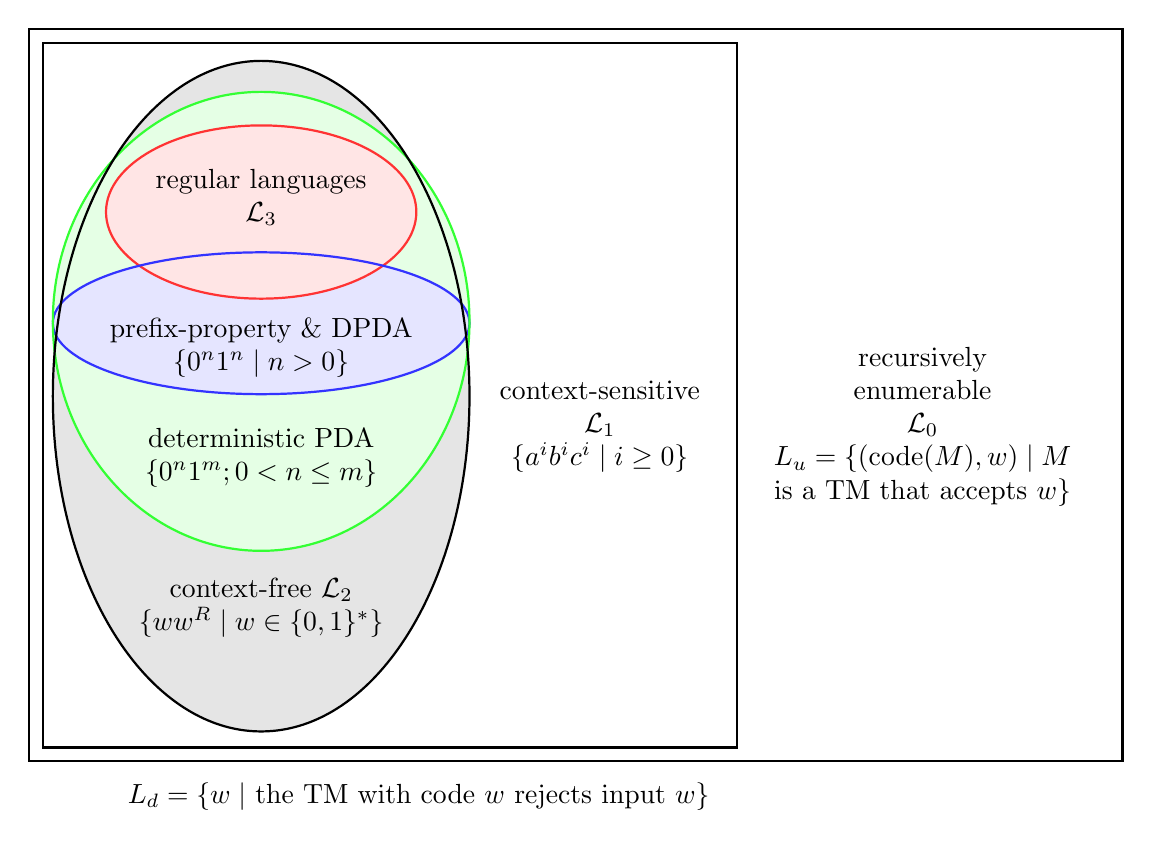
\begin{tikzpicture}[level distance=8mm]
                \node[align=center] (r1) at (1,5) {\\regular languages\\${\mathcal L}_3$};
                \node (r2) at (1,4) {};
                \node[align=center] (pref) at (1,3) {prefix-property \& DPDA\\$\{0^n1^n\mid n>0\} $};
                \node[align=center] (det) at (1,1.6) {deterministic PDA\\$\{0^n1^m; 0<n\leq m\} $};
                \node[align=center] (cfl) at (1,-0.3) {context-free ${\mathcal L}_2$\\ $\{ww^R\mid w\in \{0,1\}^*\}$};
                \node[align=center] (cl) at (5.3,2) {context-sensitive\\${\mathcal L}_1$\\$\{a^ib^ic^i\mid i\geq 0\}$};
                \node[align=center] (re) at (9.4,2) {recursively\\enumerable\\${\mathcal L}_0$
                \\$L_u=\{(\mathrm{code}(M),w)\mid M$\\ is a TM that accepts $w\}$};
                \node[align=center] (out) at (3,-2.7) {$L_d=\{w\mid$ the TM with code $w$ rejects input $w\}$};
                \node (bot) at (1,-1.6) {};
                \node (top) at (1,6.4) {};
                \node (left) at (-1.3,0) {};                
                \node[draw=red!80,thick,inner sep=-2pt,ellipse,fit=(r1) (r2) ] {};
                \node[draw=blue!80,thick,inner sep=-5pt,ellipse,fit= (r2) (pref)] {};
                \node[draw=green!80,thick,inner sep=-5pt,ellipse,fit=(r1) (r2) (pref) (det)] {};
                \node[draw=black,thick,inner sep=-5pt,ellipse,fit=(r1) (r2) (pref) (det) (cfl)] {};
                \node[draw=black,thick,inner sep=10pt,rectangle,fit=(r1) (r2) (pref) (det) (cfl) (cl) (bot) (top) (left)] {};
                \node[draw=black,thick,inner sep=15pt,rectangle,fit= (re) (bot) (top) (left)] {};                
                \begin{scope}[on background layer]
                    \node[fill=black!10,thick,inner sep=-5pt,ellipse,fit=(r1) (r2) (pref) (det) (cfl)] {};
                    \node[fill=green!10,inner sep=-5pt,ellipse,fit=(r1) (r2) (pref) (det)] {};
                    \node[fill=blue!10,thick,inner sep=-5pt,ellipse,fit= (r2) (pref)] {};
                    \node[fill=red!10,thick,inner sep=-2pt,ellipse,fit=(r1) (r2) ] {};
                \end{scope}
            \end{tikzpicture}
        }
    \end{center}      

\end{frame}


\begin{frame}{Converting between representations of context-free languages}

    \textbf{Conversions linear in input size:}
    \begin{itemize}
        \item CFG to a PDA
        \item PDA by final state to a PDA by empty stack
        \item PDA by empty stack to PDA by final state
    \end{itemize}
    
    \textbf{PDA to CFG:} $O(n^3)$ algorithm that takes a PDA $P$ whose representation has length $n$ and produces a CFG of length (sum of sizes of bodies) at most $O(n^3)$
    
    \textbf{Conversion to ChNF:} given a $\epsilon$-production-free grammar $G$ of length $n$, we can find an equivalent ChNF grammar for G in time $O(n^2)$; the resulting grammar has length $O(n^2)$

\end{frame}


\begin{frame}{Undecidable problems about context-free languages (preview)}
    
    The following problems are not algorithmically \alert{decidable}:
    \begin{itemize}
        \item Is a given context-free grammar ambiguous?
        \item Is a given context-free language inherently ambiguous?
        \item Is the intersection of two context-free languages empty?
        \item Is a given context-free language equal to $\Sigma^*$?
    \end{itemize}

\end{frame}


\begin{frame}{Summary of Lecture 8}

    \begin{itemize}
        \item Pushdown automata accept exactly context-free languages (constructions: CFG to PDA and PDA to CFG)
        \item A deterministic pushdown automaton (DPDA)
        \item DPDA recognize a proper subclass of context-free languages,\\ accepts by empty stack iff prefix-free and accepts by final state\\
        (Deterministic PDA + acceptance by empty stack does not even cover regular languages!)
        \item Deterministic PDA have unambiguous grammars
        \item The landscape of languages
        \item Converting between representations of context-free languages
        \item Undecidable problems about context-free languages (preview)
	\end{itemize}

\end{frame}


\end{document}